\chapter{Base teórica}\label{cap:teoria}
\section{Introdução}\label{sec:teoria_intro}
Dada a variedade de estudantes que podem ingressar em um curso de neurociência computacional, muitos deles podem não ter tido algumas disciplinas de base que são necessárias para um bom entendimento do conteúdo apresentado. Por isso, este capítulo contém uma base teórica útil para um nivelamento dos estudantes das mais diversas áreas. As sessões seguintes contemplam conteúdos de neurobiologia, equações diferenciais ordinárias, probabilidade e algoritmos.

\section{Neurobiologia básica}\label{sec:fisiologia}
O neurônio é a unidade básica do sistema nervoso.
%TODO: figura neurônio
É composto pelo corpo celular (chamado de soma), dendritos, que recebem sinais de outros neurônios, axônio, que transmite os sinais a serem recebidos por outros neurônios, e terminais axônicos, que são as extremidades do axônio e se conectam com os dendritos de outros neurônios. Como outras células do corpo humano, o neurônio é composto por íons e moléculas, ambas podendo possuir cargas positivas ou negativas. A célula neuronal é revestida por uma bi-camada lipídica, e geralmente o interior dela possui uma maior concentração de cargas negativas, fazendo com que o potencial de membrana ($V_m$), que é a diferença de potencial entre a parte interna e a externa da célula neuronal ($V_M=V_{dentro}-V_{fora}$), fique a maior parte do tempo com valor negativo. O potencial de membrana se altera quando há o fluxo de íons através dos poros de canais iônicos (Figura~\ref{fig:membrananeuronio}).

\begin{figure}[tb]
	\centering
	\caption[Membrana do neurônio]{Membrana do neurônio}
	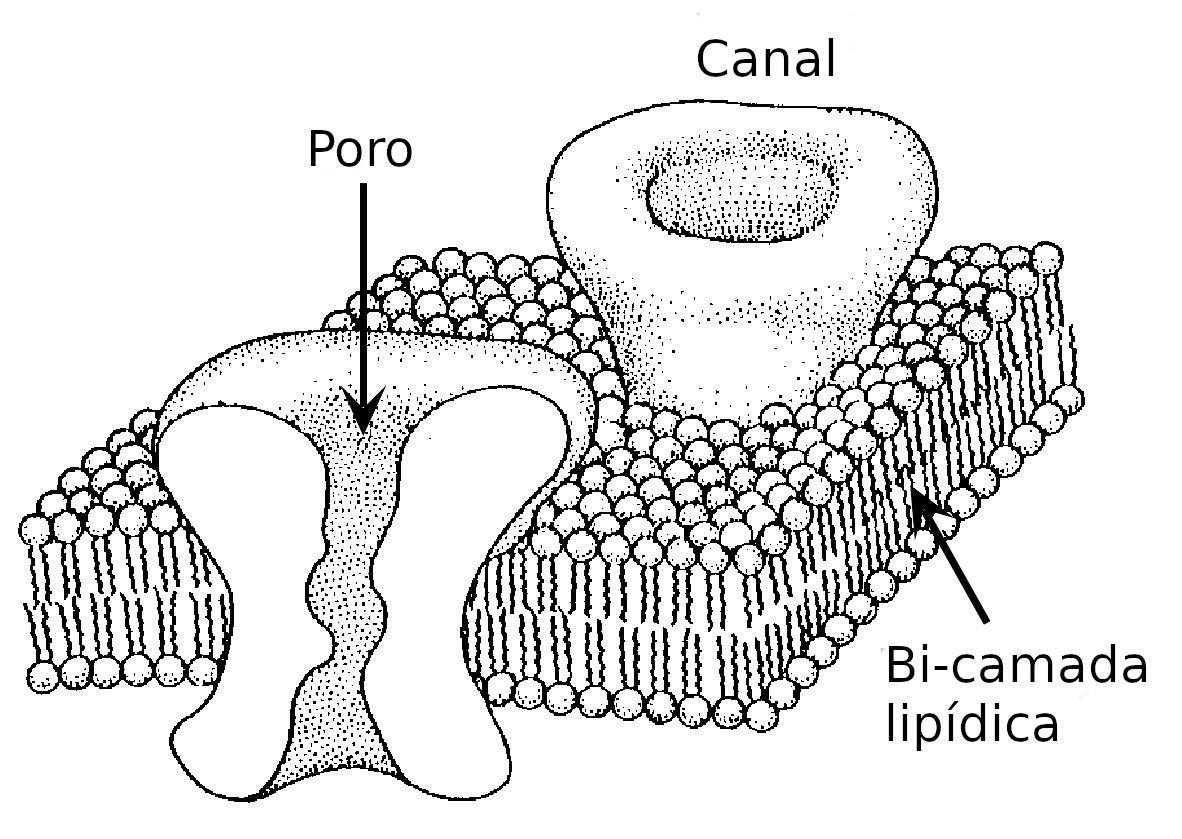
\includegraphics[width=0.55\linewidth]{figs/membrana_neuronio}
	\label{fig:membrananeuronio}
	\\
	Fonte: adaptado de \cite{hille_ionic_1992}
	%TODO: trocar figura
	%% adaptado de hille 1992 (pág. 170 pdf)
\end{figure}

Os canais iônicos são canais proteicos na membrana da célula neuronal e permitem a movimentação de íons através deles, como mostrado na Figura~\ref{fig:canaisions}. Podem ser de dois tipos: com ou sem portão. Canais sem portão estão sempre abertos, enquanto os com portão podem abrir ou fechar, dependendo do valor do potencial de membrana, e por isso são chamados de canais iônicos dependentes de tensão. Quando o fluxo de corrente elétrica de todos os íons é equilibrado dentro e fora da célula neuronal (ou seja, o potencial de membrana não se altera), ele é chamado de potencial de repouso (ou de equilíbrio). O valor típico é próximo de $-70\ mV$. O valor do potencial de repouso é calculado com base na concentração de cada íon dentro e fora da célula neuronal usando a equação de Nernst, dada por:
\begin{equation}\label{eq:nernst}
E_A=\frac{k_BT}{z_Aq_e}ln\Big(\frac{A_{fora}}{A_{dentro}}\Big)
\end{equation}
sendo $A$ o íon, $z_A$ a carga do íon, $A_{fora}$ e $A_{dentro}$ a concentração desse íon fora e dentro da célula neuronal, respectivamente, $T$ a temperatura absoluta (em Kelvin), $k_B$ a a constante de \textit{Boltzmann} ($1,39*10^{-23}\ JK^{-1}$) e $q_e$ a carga elétrica fundamental ($1,6*10^{-19}\ C$). Os valores de cargas, concentração e potencial de Nernst para alguns íons são apresentados na Tabela~\ref{tab:concentracao_nernst}.

\begin{figure}[tb!]
	\centering
	\caption[Canais iônicos de potássio]{Canais iônicos de potássio. Em \textbf{a} os íons de potássio saem da célula, causando um excesso de cargas positivas fora e negativas dentro. Em \textbf{b} o fluxo para fora e dentro é igual, causando equilíbrio}
	\label{fig:canaisions}
	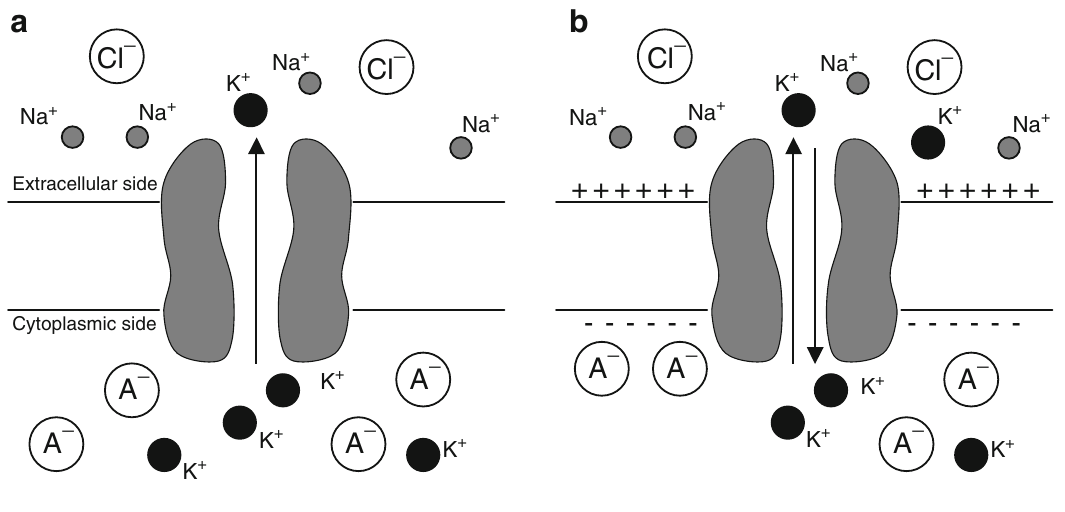
\includegraphics[width=0.7\linewidth]{figs/canais_ions}
	\\
	\cite{ermentrout_mathematical_2010}
	%TODO: trocar figura
\end{figure}

\begin{table}
	\IBGEtab{%
	\caption[Concentração de íons]{Concentração de íons}
	\label{tab:concentracao_nernst}
	}{%
	\begin{tabular}{c|c|c|c|c}
		\hline
		Íon & Carga & Conc. interna ($nM$) & Conc. externa ($nM$) & Potencial de reversão ($mV$) \\
		\hline
		Sódio & +1 & 15 & 120 & 61,6 \\
		\hline
		Potássio & +1 & 150 & 6 & -86,1 \\
		\hline
		Cloreto & -1 & 52 & 560 & -65 \\
		\hline
		Cálcio & +2 & 50 & 2 & 141,7 \\
		\hline
	\end{tabular}%
	}{
	\fonte{O autor (2023)}%
	}
\end{table}

Fora do repouso, a diferença de potencial entre o interior e o exterior do neurônio produz movimentação iônica. Quando íons positivos (como $Na^+$ ou $Ca^{2+})$ entram na célula neuronal, o potencial de membrana fica menos positivo (até próximo de 0 mV), fenômeno conhecido como despolarização. De maneira semelhante, quando íons negativos (como $K^+$) saem da célula neuronal, ou negativos (como $Cl^-$) entram, o potencial de membrana fica mais negativo, fenômeno conhecido como hiperpolarização. Os canais de potássio são mais presentes na membrana do neurônio, sendo os principais responsáveis pelo potencial de equilíbrio. Já os canais de sódio, associados à despolarização, são responsáveis pela geração do potencial de ação. Devido ao excesso de cargas negativas no interior da célula neuronal, e a existência de cargas positivas no exterior, a membrana do neurônio acaba funcionando como um capacitor, criando uma capacitância ($C_m$). O fluxo de íons através de canais sem portão é considerado constante, podendo ser agrupado em um elemento chamado de vazamento (\textit{leak}, em inglês), possuindo um potencial ($E_l$) e uma condutância ($G_l$), que é a facilidade desse elemento permitir o fluxo de corrente (o inverso da resistência). Com isso, é possível escrever uma equação relacionando o potencial de membrana da célula neuronal e os elementos de vazamento, como segue:
\begin{equation}\label{eq:potencial_membrana}
	\frac{\mathrm{d}V_m}{\mathrm{d}t}=G_l(E_l-V_m)/C_m
\end{equation}
que é dada na forma de uma equação diferencial, detalhada na seção seguinte.

\section{Equações diferenciais ordinárias}\label{sec:eqdif}
As equações diferenciais são usadas para descrever sistemas dinâmicos, ou seja, que se alteram ao longo do tempo. A forma mais básica de uma equação diferencial é:
\begin{equation}\label{eq:eq_diferencial}
	\frac{\mathrm{d}y(t)}{\mathrm{d}t}=f(y(t))
\end{equation}
com o lado esquerdo da equação sendo a derivada de $y(t)$, a função presente no lado direito associada à variável $t$, que geralmente representa o tempo. Diferentemente das equações algébricas, que possuem como solução um número, as equações diferenciais tem uma família de funções como solução, variando de acordo com a escolha de constantes, como mostrado na Figura~\ref{fig:solucao}. Nela, é exibida a família de soluções $y(t) = t + 1 + ce^t$ para a equação diferencial $y'=y-t$. $y'$ é uma representação equivalente para $\frac{\mathrm{d}y(t)}{\mathrm{d}t}$. Qualquer valor de $c$ real que for escolhido representa uma solução possível para a equação, sendo exibidas as curvas para os valores de $c$ iguais à $0$, $-1$ e $0,4$.

\begin{figure}[tb]
	\centering
	\caption{Soluções $y(t) = t + 1 + ce^t$ da equação $y'=y-t$ para vários $c$}
	\label{fig:solucao}
	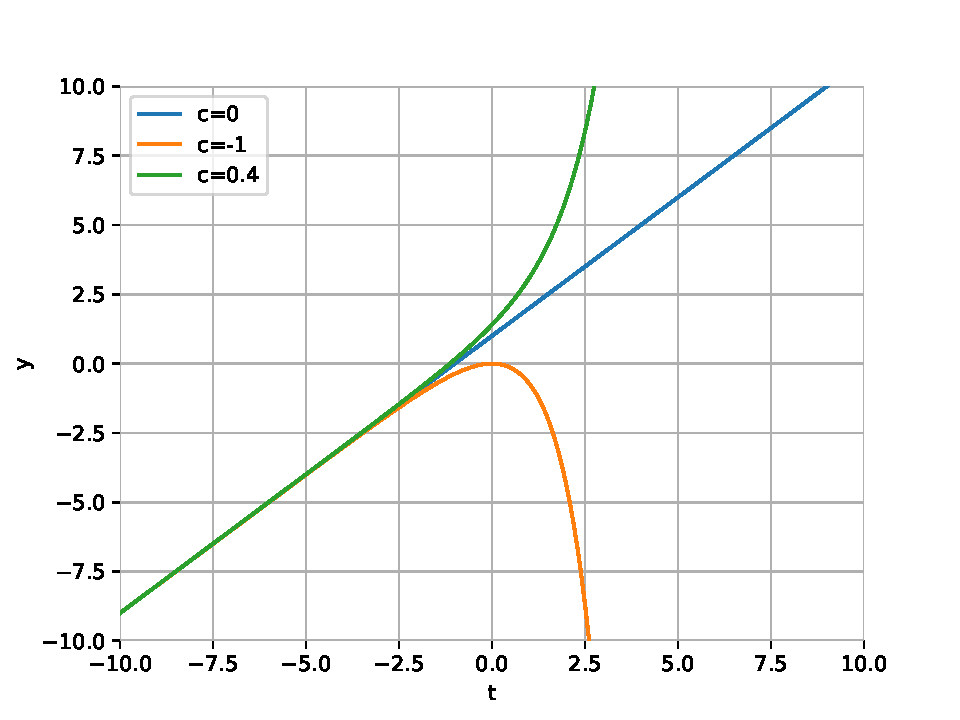
\includegraphics[width=0.7\linewidth]{figs/solucao}
	%TODO: referência
\end{figure}


\subsection{Exemplos}
\subsubsection{Decaimento radioativo}
Segundo a lei do decaimento radioativo, a taxa na qual os átomos radioativos desintegram é proporcional ao número total de átomos radioativos presente. Sendo $N(t)$ o número de átomos radioativos no tempo $t$, então $N'(t)$ é a taxa de mudança. A lei do decaimento radioativo é a que segue:
\begin{equation}\label{eq:decaimento_radioativo}
	N'(t) = -\lambda N(t)
\end{equation}
onde $\lambda$ é a constante de decaimento. Uma solução para essa equação diferencial é exibida na Figura~\ref{fig:decaimento}.

\begin{figure}[tb]
	\centering
	\caption{Decaimento radioativo ($\lambda = 0,5$)}
	\label{fig:decaimento}
	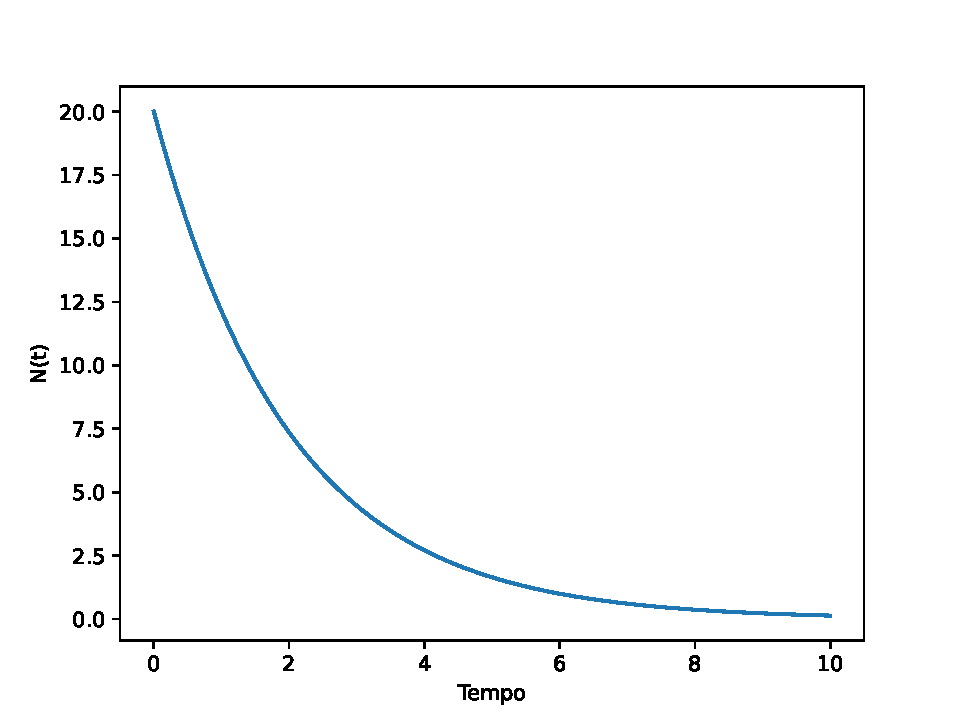
\includegraphics[width=0.6\linewidth]{figs/decaimento}
	%TODO: referência
\end{figure}

\subsubsection{Equações de Lotka-volterra}
Também conhecidas como equações predador-presa, são um par de equações diferenciais de primeira ordem, frequentemente usadas para descrever a dinâmica de sistemas biológicos de interação entre duas espécies, uma como predadora e a outra como presa. As populações de cada uma das espécies são dadas pelo par de equações:
\begin{equation}\label{eq:lotka_volterra}
	x' = ax - bxy
	$$$$
	y' = dxy - cy
\end{equation}
sendo $x$ a população da presa, $y$ a do predador, $x',\ y'$ as taxas de variação de cada população, e $a,\ b,\ c,\ d$ os parâmetros que descrevem a interação entre as espécies. A Figura~\ref{fig:lotka-volterra} exibe a solução do par de equações para um valor de cada parâmetro de interação.

\begin{figure}[tb]
	\centering
	\caption{Sistema de Lotka-Volterra ($a$ = 1,5; $b$ = 1; $c$ = 3; $d$ = 1)}
	\label{fig:lotka-volterra}
	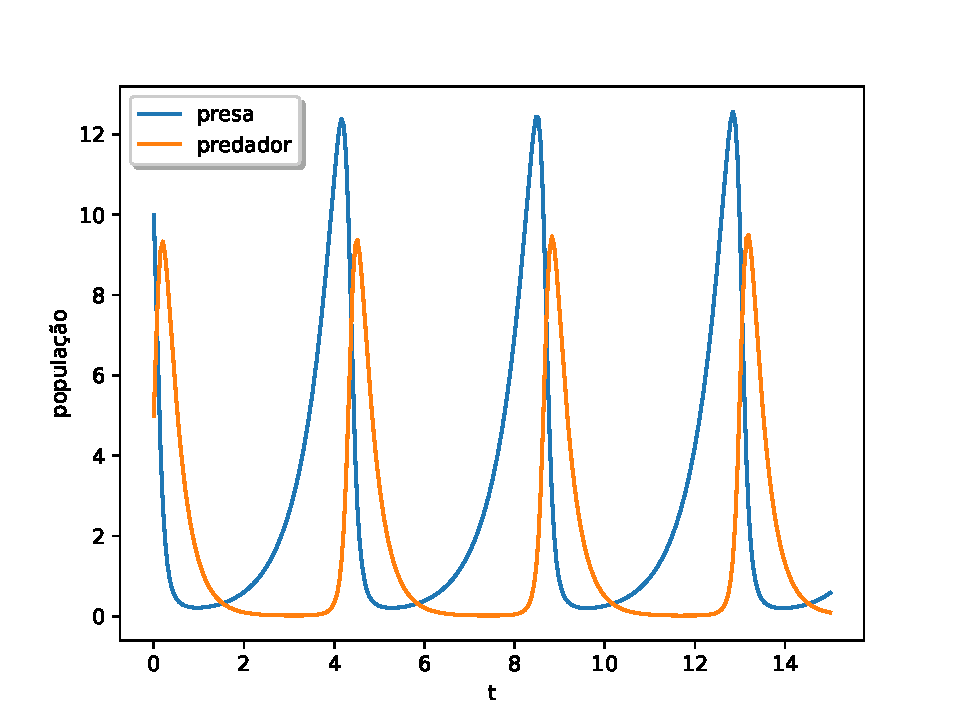
\includegraphics[width=0.6\linewidth]{figs/lotka-volterra}
	%TODO: referência
\end{figure}


%\subsubsection{Trajetória pendular}
%O pêndulo é um dispositivo que contém uma massa atrelada a um fio e que oscila em torno de um ponto fixo. A equação do movimento para o ângulo $\theta$ (o ângulo que o pêndulo faz com a vertical) é:
%
%$$
%\frac{d^2\theta}{dt^2} = -\frac{1}{Q}\frac{d\theta}{dt} + \sin{\theta} + d\cos{\Omega t}
%$$
%onde:\\
%$
%t: \text{tempo}\\
%Q: \text{fator de qualidade}\\
%d: \text{amplitude}\\
%\Omega: \text{frequência}
%$
%\\\\
%Como se trata de uma equação diferencial de segunda ordem, é necessária a redução para duas equações de primeira ordem. Fazendo a substituição de variáveis $\omega = \frac{d\theta}{dt}$ podemos reescrever da seguinte maneira:
%
%$$
%\frac{d\theta}{dt} = \omega
%$$$$
%\frac{d\omega}{dt} = -\frac{1}{Q}\omega + \sin{\theta} + d\cos{\Omega t}
%$$
%
%\begin{figure}[tb]
%	\centering
%	\caption[Trajetória pendular]{Trajetória pendular ($Q$ = 2; $d$ = 1,5; $\Omega$ = 0,65)}
%	\label{fig:pendulo}
%	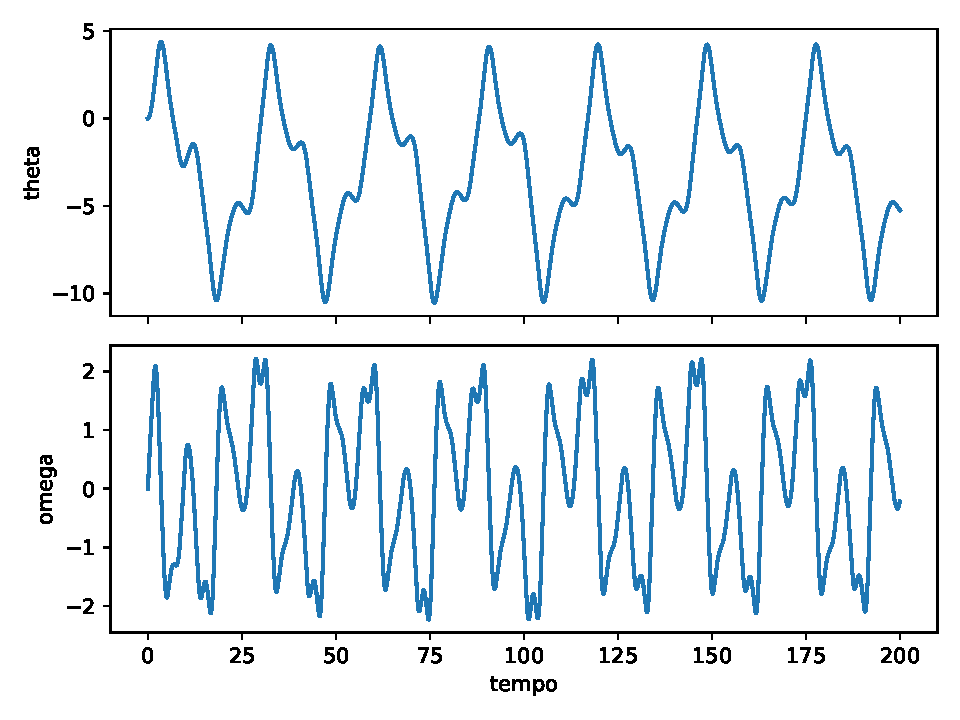
\includegraphics[width=0.7\linewidth]{figs/pendulo}
%\end{figure}

\subsection{Método de Euler}
Equações diferenciais ordinárias podem ser resolvidas analiticamente, não abordado neste texto, ou numericamente. Dentre os vários métodos existentes para a solução numérica, a adotada aqui é o método de Euler. Considerando a equação $\frac{dx}{dt}=f(x,t)$, com $f(x,t)$ uma função qualquer de $x$ em relação à $t$, dado um valor inicial $x0$ (usualmente com $t=0$), é possível simular a equação usando pontos discretos com intervalos $\Delta t$ fixos. Cada valor $x_n$ é dado por $x_n=x(t_n=n\Delta t)$. A partir disso, é possível usar o método de Euler avançado para calcular um valor seguinte a partir do valor anterior, ou seja:
$$
x_{n+1}=x_n+f(x_n,t_n)\Delta t
$$
como é demonstrado na Figura~\ref{fig:euler}. Outros métodos não abordados no curso incluem o método de Euler reverso e o Runge-Kutta de segunda e quarta ordens, que são mais precisos na solução. O algoritmo (sequência de instruções para executar uma determinada tarefa) do método de Euler será implementado usando a linguagem Python, que tem a sua base detalhada no Apêndice~\ref{ap:python}.
\begin{figure}[tb]
	\centering
	\caption{Método de Euler}
	\label{fig:euler}
	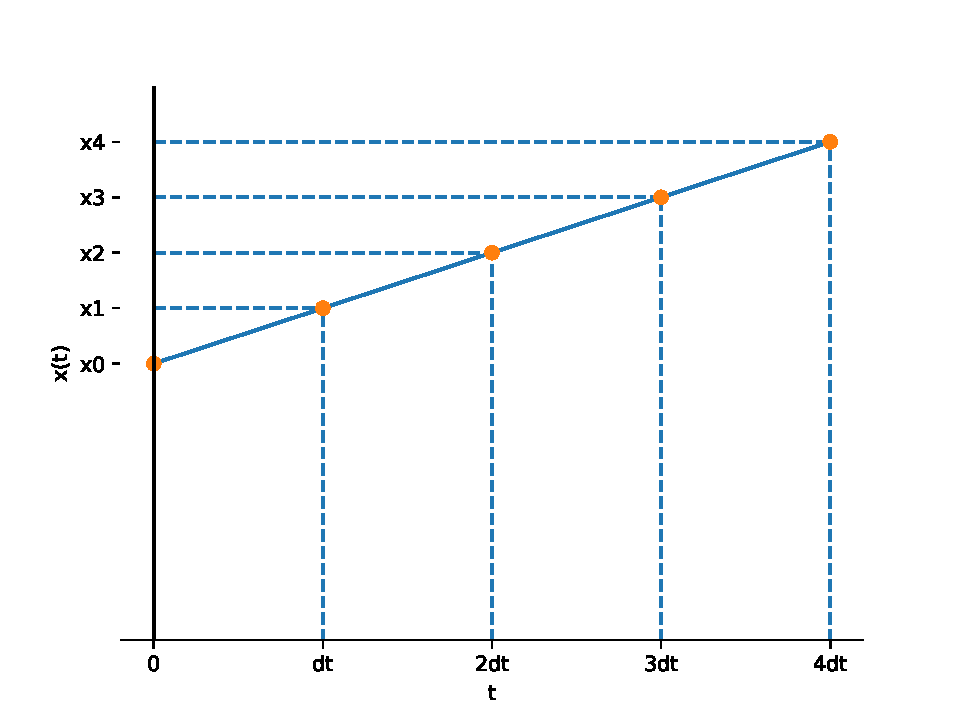
\includegraphics[width=0.7\linewidth]{figs/euler}
	%TODO: referência
\end{figure}


%\section{Probabilidade}\label{sec:probabilidade}
%\begin{itemize}
%	\item Experimento aleatório: pode fornecer resultados diferentes a cada vez que se repete da mesma maneira
%	\item Espaço amostral (S): conjunto de resultados possíveis para um experimento aleatório (pode ser contínuo ou discreto)
%	\item Espaço amostral discreto: conjunto finito ou infinito contável de resultados
%	\item Espaço amostral contínuo: intervalo (finito ou infinito) de números reais
%	\item Evento (E): subconjunto do espaço amostral
%\end{itemize}
%
%
%\subsection{Probabilidade}
%\begin{itemize}
%	\item Probabilidade: quantifica a chance de ocorrer o resultado de um experimento aleatório (“A chance de chover hoje é de 30\%")
%	\item Axiomas:
%	\begin{enumerate}
%		\item $P(S)=1$
%		\item $0\leq P(E)\leq 1$
%		\item $E_1\cap E_2=\emptyset\to P(E_1)+P(E_2)$
%	\end{enumerate}
%	\item Probabilidade da união: $P(A\cup B)=P(A)+P(B)-P(A\cap B)$
%	\item Probabilidade condicional: $P(B|A)=P(A\cap B)/P(A),\quad P(A)>0$
%	\item Teorema de Bayes:  $P(A|B)=\frac{P(B|A)P(A)}{P(B)},\quad P(B)>0$\\ % ex. do teste de droga
%	\begin{description}
%		\item[Exemplo:] Pelo fato de um novo procedimento médico ter se mostrado efetivo na detecção prévia de uma doença, propôs-se um rastreamento médico da população. A probabilidade de o teste identificar corretamente alguém com a doença, dando positivo, é $0,99$, e a probabilidade de o teste identificar corretamente alguém sem a doença, dando negativo, é $0,95$. A incidência da doença na população em geral é $0,0001$. Você fez o teste e o resultado foi positivo. Qual é a probabilidade de você ter a doença?
%		\item[Solução:] Seja $D$ o evento em que você tem a doença e seja $S$ o evento é que o teste é positivo. A probabilidade requerida pode ser denotada como $P(D|S)$. A probabilidade de o teste identificar corretamente alguém sem a doença, dando negativo, é $0,95$. Consequentemente a probabilidade de um teste positivo sem a doença é
%		$$P(S|D') = 0,05$$
%		Do Teorema de Bayes,
%		\begin{align*}
%			P(D|S)&=P(S|D)P(D)/[P(S|D)P(D)+P(S|D')P(D')]\\
%			&=0,99*0,0001/[0,99*0,0001+0,05*(1-0,0001)]\\
%			&=1/506=0,002
%		\end{align*}
%		\item[Interpretação Prática:] A probabilidade de você ter a doença da de um resultado positivo do teste é somente 0,002. Surpreendentemente, embora o teste seja efetivo, no sentido de que $P(S|D)$ é alto e $P(S|D')$ é baixo, por causa da incidência da doença na população em geral ser baixa, as chances são bem pequenas de você realmente ter a doença, mesmo se o teste for positivo
%	\end{description}
%\end{itemize}
%
%
%\subsection{Variáveis aleatórias}
%\begin{itemize}
%	\item Variável aleatória ($X$): função que atribui um número real ($x$) a cada resultado no espaço amostral de um evento aleatório
%	\item Discretas: número de pessoas adultas em um ambiente; numero de carros em uma rodovia
%	\item Contínuas: corrente elétrica; temperatura; tempo
%	\item Função densidade de probabilidade discretas:
%	\begin{enumerate}
%		\item $f(x_i) \geq 0$ (para todo $x$)
%		\item $\sum_{i=1}^n f(x_i)=1$
%		\item $f(x_i)=P(X=x_i)$
%	\end{enumerate}
%	\item Função de distribuição cumulativa discretas: $F(x)=P(X\leq x)=\sum_{x_i\leq x}f(x_i)$
%	\begin{enumerate}
%		\item $0\leq F(x)\leq 1$
%		\item Se $x\leq y$, então $F(x)\leq F(y)$
%	\end{enumerate}
%	\item Função densidade de probabilidade contínuas:
%	\begin{enumerate}
%		\item $f(x) \geq 0$ (para todo $x$)
%		\item $\int_{-\infty}^\infty f(x)\mathrm{d}x=1$
%		\item $P(a\leq X\leq b)=\int_a^b f(x)\mathrm{d}x=$ área sob $f(x)$ de $a$ a $b$ para qualquer $a$ e $b$
%	\end{enumerate}
%	\item Função de distribuição cumulativa contínuas: $F(x)=P(X\leq x)=\int_{-\infty}^{x}f(u)\mathrm{d}u$
%\end{itemize}
%\subsubsection{Média e variância}
%\begin{itemize}
%	\item Média (valor esperado) de uma variável aleatória discreta: $\mu=E(X)=\sum_{x}xf(x)$
%	\item Variância de uma variável aleatória discreta: $\sigma^2=V(X)=E(X-\mu)^2$ (desvio-padrão: $\sigma=\sqrt{\sigma^2}$)
%	\item Média (valor esperado) de uma variável aleatória contínua: $\mu=E(X)=\int_{\infty}^{\infty}xf(x)\mathrm{d}x$
%	\item Variância de uma variável aleatória contínua: $\sigma^2=V(X)=\int_{-\infty}^{\infty}x^2f(x)\mathrm{d}x-\mu^2$ (desvio-padrão: $\sigma=\sqrt{\sigma^2}$)
%\end{itemize}
%
%\subsubsection{Distribuição de Poisson}
%$$
%f(x)=\frac{e^{-\lambda T}(\lambda T)^x}{x!}, x=0,1,2,\dots
%$$
%\begin{itemize}
%	\item $T$: intervalo do evento
%	\item $\lambda$: número médio de eventos por intervalo ($0\leq\lambda$)
%	\begin{description}
%		\item[Exemplo:] Falhas ocorrem ao acaso ao longo do comprimento de um fio delgado de cobre. Suponha que o número de falhas siga a distribuição de Poisson, com uma média de 2,3 falhas por milímetro. Determine a probabilidade de existirem exatamente duas falhas em 1 milímetro de fio.
%		\item[Solução:] Seja $X$ o número de falhas em 1 milímetro de fio. Então, $E(X)=2,3$ falhas e
%		$$P(X=2) = \frac{e^{-2,3}(2,3)^2}{2!}=0,265$$
%		Para determinar a probabilidade de 10 falhas em 5 milímetros de fio, consideramos $X$ o número de falhas em 5 milímetros de fio. Então, $X$ tem uma distribuição de Poisson com
%		$$\lambda T=5\text{ mm X }2,3\text{ falhas/mm}=11,5\text{ falhas}$$
%		Consequentemente,
%		$$P(X=10)=e^{-11,5}\frac{(11,5)^{10}}{10!}=0,113$$
%		\item[Interpretação Prática:] Dadas as suposições para um processo de Poisson e um valor para $\lambda$, as probabilidades podem ser calculadas para intervalos arbitrários de comprimento.
%	\end{description}
%\end{itemize}
%
%\subsubsection{Distribuição normal (Gaussiana)}
%$$
%f(x)=\frac{1}{\sqrt{2\pi\sigma}}e^{\frac{-(x-\mu)^2}{2\sigma^2}}\qquad-\infty<x<\infty
%$$
%
%$$
%E(X)=\mu\qquad V(X)=\sigma^2
%$$
%
%\begin{figure}[htb!]
%	\centering
%	\caption{Funções densidade de probabilidade normal para diferentes valores de $\mu$ e $\sigma^2$}
%	\label{fig:normal}
%	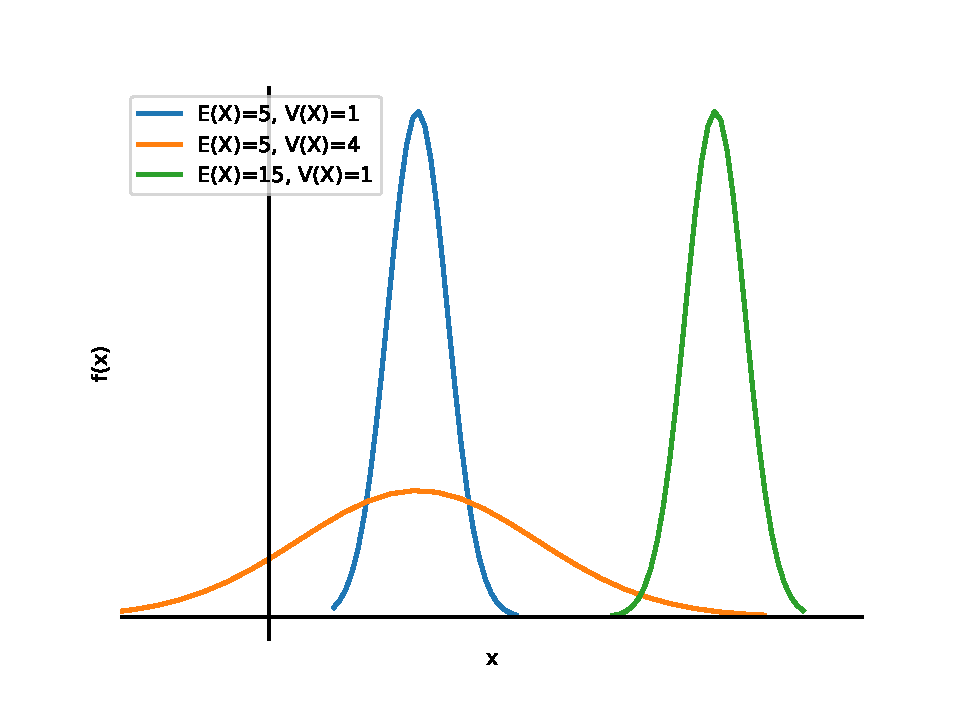
\includegraphics[width=0.7\linewidth]{figs/normal}
%\end{figure}
%
%
%\begin{itemize}
%	\item Normal padrão: $\Phi(z)=P(Z\leq z)$, quando $\mu=0$ e $\sigma=1$
%\end{itemize}

%
%\section{Noções de algoritmos e programação}\label{sec:algoritmo}
%\begin{itemize}
%	\item \textbf{Algoritmo}: sequência de instruções para executar uma determinada tarefa. Ex.: algoritmo para lavar as mãos
%	\begin{enumerate}
%		\centering
%		\item Início
%		\item Abrir a torneira
%		\item Molhar as mãos
%		\item Ensaboar as mãos
%		\item Molhar as mãos
%		\item Secar as mãos
%		\item Fim
%	\end{enumerate}
%	
%	\item \textbf{Programa}: conjunto de instruções escritas em um arquivo com regras específicas
%	\begin{verbatim}
%		print("Olá, mundo!")
%	\end{verbatim}
%	\item \textbf{Linguagem de programação}: converte o programa escrito em ações no computador (ex.: \textit{Python}, \textit{C++}, \textit{Java})
%\end{itemize}
%
%\begin{figure}[htb!]
%	\centering
%	\caption{Do código para e/s}
%	\label{fig:codigoio}
%	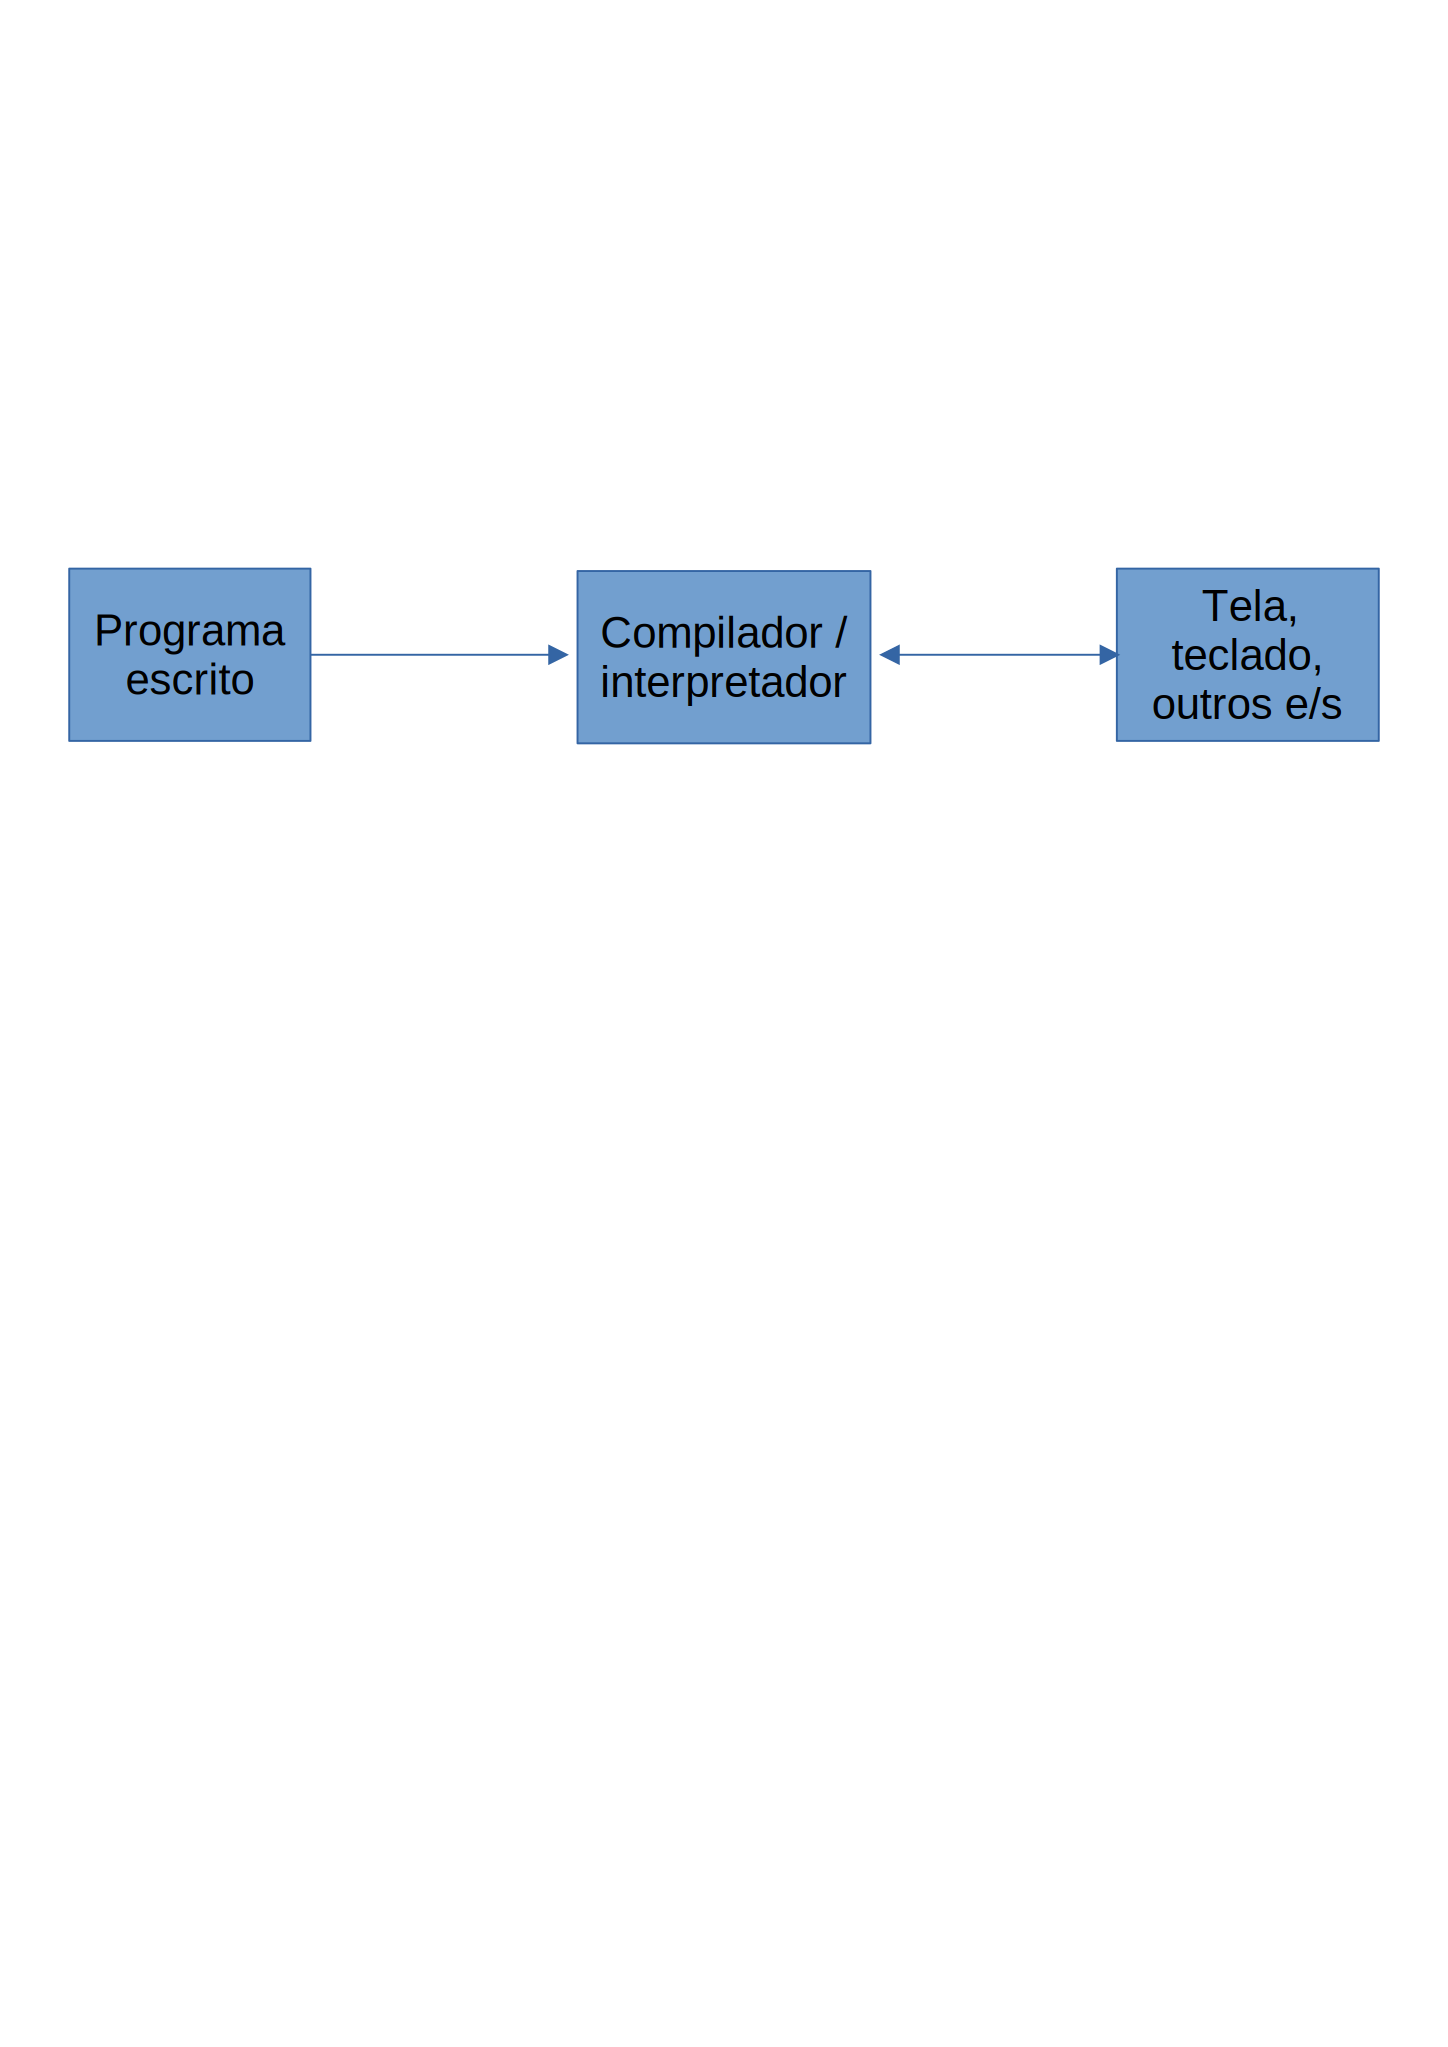
\includegraphics[width=0.7\linewidth]{figs/codigo_io}
%\end{figure}
%
%\SetKwComment{Comment}{/* }{ */}
%\begin{algorithm}
%	\caption{Exemplo}\label{alg:ohm}
%	\KwData{$n \geq 0$}
%	\KwResult{$y = x^n$}
%	$y \gets 1$\;
%	$X \gets x$\;
%	$N \gets n$\;
%	\While{$N \neq 0$}{
%		\eIf{$N$ é par}{
%			$X \gets X \times X$\;
%			$N \gets \frac{N}{2}$ \Comment*[r]{Este é um comentário}
%		}{\If{$N$ é impar}{
%				$y \gets y \times X$\;
%				$N \gets N - 1$\;
%			}
%		}
%	}
%\end{algorithm}
